\documentclass[a4paper,12pt]{report}
%\documentclass[a4paper,10pt]{scrartcl}

\usepackage[utf8]{inputenc}
\usepackage[french]{babel}
\usepackage[T1]{fontenc}
\usepackage{graphicx}
% \usepackage{hyperref}
\usepackage{tikz}
\usepackage[margin=0.75in]{geometry}
\usetikzlibrary{arrows}

\renewcommand{\chaptername}{}
\setcounter{chapter}{-1}

\tikzset{
  treenode/.style = {align=center, inner sep=0pt, text centered,
    font=\sffamily},
  arn_n/.style = {treenode, circle, draw=black, text width=2em},
  arn_x/.style = {treenode, rectangle, draw=black, text width=1.5em,
    minimum width=1.5em, minimum height=1.5em}
}

\title{\Huge Rapport \\ Projet ALGAV Trie \\ \large Implantation du Trie Hybride et du Patricia Trie}
\author{Amel Arkoub 3301571 \\ Ling-Chun SO 3414546}
\date{22 décembre 2017}

\pdfinfo{%
  /Title    ()
  /Author   ()
  /Creator  ()
  /Producer ()
  /Subject  ()
  /Keywords ()
}

\begin{document}
\maketitle

\tableofcontents
\newpage

\chapter{Introduction}
\section*{Présentation}
\paragraph*{}
Nous souhaitons représenter un dictionnaire de mots, c'est-à-dire implanter une structure de
données efficace stockant des mots. Pour cela, nous allons nous servir de la structure de {\itshape trie}.
Dans cette optique, nous proposons les implantations de deux structures de tries concurrentes : le trie hybride
et le PATRICIA trie. Ensuite, nous effectuerons une étude expérimentale de laquelle nous analyserons les résultats, afin de mettre en exergue
les avantages et inconvénients de chacune des structures. Nous avons choisi le langage de programmation Java pour nos implantations.

\section*{Trie}
Un trie est une représentation arborescente d'un ensemble de clés qui permet d'éviter la répétition de préfixes communs des mots.

\section*{Trie Hybride}
Un trie hybride est un arbre ternaire dont chaque nœud contient un caractère et une valeur (non vide
lorsque le nœud représente une clé). Chaque nœud a 3 pointeurs: un lien Inf (resp. Eq, res. Sup) vers le sous-arbre dont le premier caractère est inférieur (resp. égal, resp. supérieur) à son caractère. Il permet en outre
de réduire le nombre de pointeurs vides par rapport à un R-Trie.

\section*{PATRICIA Trie}
Un PATRICIA trie est un arbre dont le but est de réduire la hauteur des R-Trie tout en conservant une recherche
efficace. Pour ce faire, plutôt que chaque nœud interne ait pour valeur une lettre, il a pour valeur le préfixe commun à un ensemble de mots.

\chapter{Trie Hybride}
\section{Implantation}
\subsection{Structure}
Dans notre implantation JAVA, un trie hybride est un objet qui contient 5 éléments:
\begin{itemize}
 \item un char ``letter'', qui correspond à la lettre stockée.
 \item une valeur ``value'', qui correspond à la représentation de fin de mot (-1 le nœud n'est pas la fin
 d'un mot, sinon la valeur correspond à l'ordre d'ajout croissant).
 \item un pointeur vers un trie hybride ``fc'', ce trie hybride correspond au fils central, c'est-à-dire on parcours ce
 trie hybride si le caractère recherché au Trie Hybride courant est correct.
 \item un pointeur vers un trie hybride ``fg'', ce trie hybride correspond au fils gauche, c'est-à-dire on parcours ce
 trie hybride si le caractère recherché au Trie Hybride courant est plus petit dans l'ordre alphabétique.
 \item un pointeur vers un trie hybride ``fd'', ce trie hybride correspond au fils droit, c'est-à-dire on parcourt ce
 trie hybride si le caractère recherché au trie hybride courant est plus grand dans l'ordre alphabétique.
\end{itemize}

\paragraph*{}
Voici une représentation du trie hybride résultant des ajouts successifs des mots:
\begin{itemize}
 \item don
 \item le
 \item a
 \item dort
\end{itemize}

\begin{tikzpicture}[->,>=stealth',level/.style={sibling distance = 6cm/#1,
  level distance = 2.5cm}]
\node [arn_n] {d \\ -1}
    child{ node [arn_n] {a \\ 2}}
    child{ node [arn_n] {o \\ -1}
	    child{ node [arn_x] {}}
            child{ node [arn_n] {n \\ 0} 
							child{ node [arn_n] {r \\ -1}
							      child{ node [arn_n] {t \\ 3}}
							}
							child{ node [arn_x] {}}
							child{ node [arn_x] {}}
            }
            child{ node [arn_x] {}}
		}
    child{ node [arn_n] {l \\ -1}
	    child{ node [arn_n] {e \\ 1}}
    }
; 
\end{tikzpicture}
\begin{figure}[!htbp]
\caption{Représentation d'un Trie Hybride}
\end{figure}

\section{Description des algorithmes}
\subsection{Algorithmes triviaux}
La plupart des algorithmes de l'implantation du trie hybride sont relativement triviaux, notamment
les fonctions:
\begin{itemize}
 \item Recherche(arbre, mot) $\rightarrow$ booléen
 \item ComptageMots(arbre) $\rightarrow$ entier
 \item ListeMots(arbre) $\rightarrow$ liste[mots]
 \item ComptageNil(arbre) $\rightarrow$ entier
 \item Hauteur(arbre) $\rightarrow$ entier
 \item ProfondeurMoyenne(arbre) $\rightarrow$ entier
 \item Prefixe(arbre) $\rightarrow$ entier
\end{itemize}
Elles correspondent pour la plupart d'un simple parcours de la structure du trie hybride, dont le traitement
dépend de la fonction.

\subsection{AjoutMot}
La fonction ajoutMot permet d'ajouter un mot dans le trie hybride, et par conséquent la construction même du trie hybride,
dont la signature est: ajoutMot(mot, arbre) $\rightarrow$ void.
Les étapes sont donc:
\begin{itemize}
 \item le cas d'arrêt lorsque le mot a été ajouté.
 \item si on est dans la racine qui est encore vide alors on ajoute le mot.
 \item si le mot est de longueur 1, alors on vérifie si le trie hybride courant correspond à la bonne lettre
 sinon on fait des appels récursifs sur le fils gauche ou droit.
 \item dans le cas général, on compare le caractère du mot et le caractère du trie hybride courant, si les lettres
 concordent alors on appelle récursivement sur le fils central ; si elles sont différentes, on fait un appel récursif sur le
 fils gauche ou droit suivant l'ordre alphabétique des caractères.
\end{itemize}

\subsection{Suppression}
La fonction suppressionMot permet la suppression d'un mot dans le trie hybride et maintient le trie hybride cohérent en supprimant
les nœuds dont il n'existe pas de mot, la signature est: suppression(arbre, mot) $\rightarrow$ void
Les étapes sont donc:
\begin{itemize}
 \item si le trie hybride courant est un pointeur null alors on a un cas d'arrêt.
 \item si le mot est réduit à une lettre alors on vérifie que le caractère du mot et du trie hybride courant sont égaux. Dans ce cas, on ne considère plus le trie hybride comme un mot. Dans le cas contraire, c'est-à-dire s'ils ne sont
 pas égaux, alors on fait un appel récursif sur le fils gauche ou droit suivant la comparaison de l'ordre alphabétique des lettres.
 \item dans le cas général, on compare le caractère du mot et le caractère du Trie Hybride courant, si les lettres
 concordent alors on appelle récursivement sur le fils central ; si elles sont différentes, on fait un appel récursif sur le
 fils gauche ou droit suivant l'ordre alphabétique des caractères.
 \item on calcul le nombre de mots issus de chaque fils, s'il existe un fils dont le nombre de mots est égal à 0, alors on détruit
 le fils en question.
\end{itemize}


\section{Complexité}
\subsection{Recherche}
Pour la recherche d'un mot de \textit{L} caractères et un trie hybride de taille \textit{n}, 
en prenant la comparaison de caractère comme mesure, on obtient une complexité dans le cas général:
\begin{itemize}
 \item en $\Theta$(L), si \textit{L} < \textit{n};
 \item en $\Theta$(n) sinon.
\end{itemize}
Sinon on a une complexité en $\Theta$(n) dans le pire cas.

\subsection{Comptage Mots}
Le comptage de mots revient à faire un parcours de l'arbre en entier.
Soit un arbre de taille \textit{n}, en prenant la comparaison de la valeur du nœud comme mesure,
on a donc une complexité $\Theta$(n).

\subsection{Liste Mots}
La récupération des mots dans un trie hybride correspond aussi à un parcours de l'arbre en entier en gardant le \textit{préfixe}
en argument dans les appels de fonctions.
Soit un arbre de taille \textit{n}, en prenant la comparaison de la valeur du nœud comme mesure,
on a donc une complexité en $\Theta$(n).

\subsection{Comptage Nil}
Le comptage de pointeur vers null correspond à un parcours de tous les nœuds pour compter le nombre de fils null.
Soit un arbre de taille \textit{n}, en prenant la comparaison de la valeur du nœud comme mesure,
on a une complexité en $\Theta$(n) puisque pour \textit{n} noeuds, on a un nombre de comparaisons $\le$ \textit{3n}.

\subsection{Hauteur}
La détermination de la hauteur du trie hybride est un parcours complet de l'arbre, en prenant l'existence de fils comme mesure, on obtient une complexité en $\Theta$(n).

\subsection{Profondeur Moyenne}
La profondeur moyenne d'un trie hybride est un parcours jusqu'aux feuilles dont on ajoute la profondeur dans une liste et on effectue
une division. En prenant la comparaison d'existence de fils comme mesure, on obtient une complexité de $\Theta$(n).

\subsection{Préfixe}
La recherche du préfixe peut être dans le pire cas en $\Theta$(n). En effet, le pire cas est atteint lorsque le trie hybride
est une ``liste chaînée'' et donc à hauteur \textit{h}=n.

\subsection{Suppression}
La suppression d'un mot est une recherche dans le trie hybride, ce qui correspond à une complexité en $\Theta$(n) comparaisons
dans le pire cas. Cependant, il y a aussi 3 appels à la fonction comptageMots de complexité $\Theta$(n).
On a donc une complexité en $\mathcal{O}$($n^2$).

\chapter{Patricia Trie}
\section{Implantation}
Dans notre implantation JAVA, un PATRICIA trie est représenté par :
\begin{itemize}
\item une chaîne de caractères, nommée {\itshape valeur}, qui est le préfixe.
\item un tableau de 27 PATRICIA tries fils {\itshape patTries}, un pour chaque lettre de l'alphabet, le 27ème représentant le caractère de fin de mot. Ce caractère est "\{" .
\item un indice, entier nommé {\itshape ind}, qui est le numéro de la prochaine lettre à évaluer dans les mots fils. En effet, les mots fils ont ce même préfixe, et diffèrent à partir de la lettre indiquée par l'indice.
\item un booléen, {\itshape isFeuille} indiquant si ce nœud est une feuille ou non. Dans le cas où le nœud est une feuille, le préfixe est en fait le mot en entier.
\end{itemize}
 \bigbreak
AJOUTER SCHÉMA PAT TRIE

\section{Complexité}
\subsection{Recherche}
La recherche d'un mot dans un PATRICIA trie de hauteur h est de complexité O(h).
En effet, lors de la recherche, on est aiguillé par l'indice du PATRICIA trie, qui nous mène vers un de ses PATRICIA trie fils.

\subsection{Comptage Mots}
Soit un PATRICIA trie de taille n. Compter les mots qu'il contient revient à parcourir chaque nœud de l'arbre. Ainsi sa complexité est $\Theta$(n).

\subsection{Liste Mots}
Soit un PATRICIA trie de taille n. Lister les mots qu'il contient revient à parcourir chaque nœud de l'arbre. Ainsi sa complexité est $\Theta$(n).

\subsection{Comptage Nil}
Soit un PATRICIA trie de taille n. Compter le nombre de pointeurs à nil qu'il contient revient à compter le nombre de pointeurs à nil de chaque nœud de l'arbre. Ainsi sa complexité est $\Theta$(n).

\subsection{Hauteur}
Soit un PATRICIA trie de taille n. Pour trouver sa hauteur, il faut parcourir chaque branche de l'arbre. Ainsi, on parcourt chaque nœud qu'il contient. Ainsi sa complexité est $\Theta$(n).

\subsection{Profondeur Moyenne}
Soit un PATRICIA trie de taille n. Pour trouver sa profondeur moyenne, il faut parcourir chaque branche de l'arbre, et récupérer toutes les longueurs de ses branches, et ensuite en faire la moyenne ( en O(1) ). Ainsi, on parcourt chaque nœud qu'il contient. Ainsi sa complexité est $\Theta$(n).

\subsection{Préfixe}
Soit un PATRICIA trie de taille n. Pour le nombre de mots qui ont en commun un certain préfixe, il faut parcourir la branche de l'arbre qui contient ce préfixe,. Ainsi, on parcourt chaque nœud qu'il contient. Ainsi sa complexité est $\Theta$(n).
\subsection{Suppression}

\chapter{Fonctions complexes}
\section{Implantation}
\subsection{Fusion de Patricia Trie}

\subsection{Conversion de Patricia Trie en Trie Hybride}

\subsection{Conversion de Trie Hybride en Patricia Trie}

\subsection{Rééquilibrage de Trie Hybride}
\paragraph{}
Après plusieurs ajouts successifs dans un trie hybride, ce dernier peut être plutôt déséquilibré. Nous avons donc implanté
une fonction permettant d'identifier si un trie hybride est équilibré et le rééquilibrage de celui-ci dans le cas contraire.
Nous remarquons dans un trie hybride qu'il n'est pas modifiable dans la profondeur des fils centraux mais qu'il l'est à
partir d'un nœud courant, pour ses fils gauche et droit. En effet, ceux-ci sont ``intervertibles'' entre eux, nous pouvons donc
considérer comme un équilibrage d'AVL dont les fils gauche et droit correspondent respectivement aux fils gauche et droit d'un AVL.
La fonction checkBalance(arbre) $\rightarrow$ booléen, permet d'identifier si un trie hybride est équilibré ou non. Celle-ci
calcule dans tout le trie hybride s'il existe un nœud dont le nombre de successions de fils gauche ou droit dans le fils gauche ou 
droit du nœud courant diffère de plus de 1. Si tel est le cas, alors le trie hybride est déséquilibré.

\paragraph{}
La fonction de rééquilibrage est balanceTrieHybride(arbre) $\rightarrow$ void, elle se décompose en ces étapes:
\begin{itemize}
 \item le cas de base est le trie hybride est null.
 \item on calcule si le trie hybride est déjà équilibré : s'il est équilibré alors on récupère tous les fils centraux de la
 successions de fils gauche et droit du nœud courant et on effectue des appels recursifs sur ces fils.
 \item on extrait la succession des fils gauche et droit du nœud courant et on effectue un tri dans l'ordre alphabétique
 \item on retire dans ces nœuds les liens fils gauche et droit
 \item on calcule le nœud qui sera au milieu, l'élément qui coupe en deux sous tableaux de taille égal
 \item étant donné que nous manipulons des pointeurs et ne possédant pas de pointeur sur le père, nous remplaçons le contenu
 dans l'ancien nœud courant par le nouveau nœud milieu, et vice-versa.
 \item on effectue un appel à la fonction splitting(arbre,arbre[],arbre[]), celui-ci permet pour un nœud courant d'attribuer le
 fils gauche et droit. le premier tableau correspond a l'ensemble des fils gauches que peut prendre le nœud courant et le second
 tableau correspond à l'ensemble des fils droits que peut prendre le nœud courant. Ainsi cette fonction récursive calcule par
 dichotomie les fils gauche et droit des nœuds.
 \item on récupère tous les fils centraux du chemin de fils gauche et droit pour faire des appels récursifs
\end{itemize}
Il est important de noter que le nombre maximal de nœuds d'un chemin de fils gauche et droit est majoré par une constante (26
pour les lettres de l'alphabet).

\section{Complexité}
\subsection{Fusion de Patricia Trie}

\subsection{Conversion de Patricia Trie en Trie Hybride}

\subsection{Conversion de Trie Hybride en Patricia Trie}

\subsection{Rééquilibrage de Trie Hybride}
\paragraph{checkBalance}
La fonction qui vérifie si un trie hybride est équilibré s'appuie sur la fonction checkBalanceAux, qui elle-même fait appel à la fonction countLRNode.
Les complexités sont donc:
\begin{itemize}
 \item countLRNode est en $\Theta$(26) donc en $\Theta$(1), car le plus long chemin des fils gauche et droit est majoré par 26
 \item checkBalanceAux est donc aussi en $\Theta$(1), puisque cette fonction calcule pour les fils gauche et droit du nœud courant
 \item checkBalance est en $\Theta$($\log_{26}$(n)) donc en $\Theta$($\log_{}$(n)), puisqu'elle fait appel à checkBalanceAux 
pour tous les nœuds sauf les nœuds du chemin des fils gauche et droit.
\end{itemize}

\paragraph{balanceTrieHybride}
De la même manière que checkBalance, la fonction balanceTrieHybride est en $\Theta$($\log_{}$(n)), puisque toutes les opérations
sont des opérations en $\Theta$(1) sauf pour les appels récursifs.

\chapter{Etude expérimentale}
\section{Temps de construction}
Nous avons calculé le temps de construction des différentes implantations réalisées. Nous avons chargé avec un pas de 1000,
tous les mots contenus dans l’œuvre de Shakespeare, en repartant d'un trie vide à chaque pas.\\
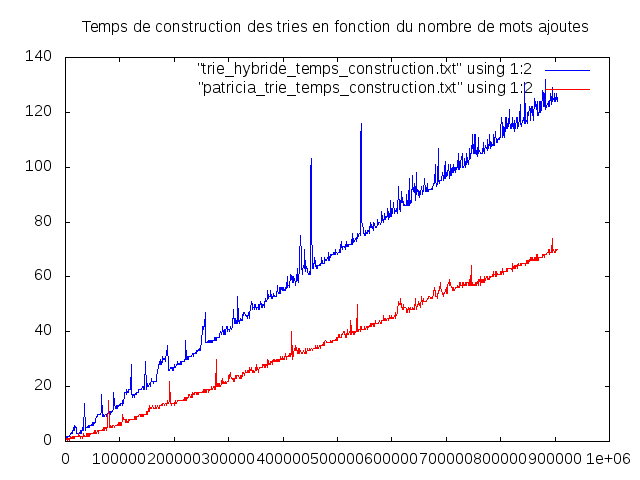
\includegraphics{../comparaison/courbe_temps_construction.png}
\begin{figure}[!htbp]
\caption{Courbe du temps de calcul en fonction du nombre d'ajouts}
\end{figure}

\section{Temps d'ajout d'un mot}
Nous avons aussi calculé le temps d'ajout d'un mot dans des tries qui avaient les œuvres de Shakespeare déjà chargées. Nous avons alors
ajouté des mots français de longueur croissante, dont le plus long mot est composé de 25 lettres.\\
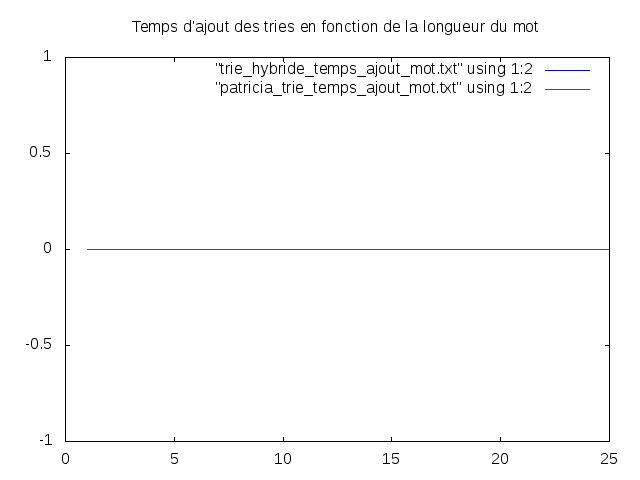
\includegraphics{../comparaison/courbe_ajout_mot.png}
\begin{figure}[!htbp]
\caption{Courbe du temps de calcul en fonction de la longueur du mot}
\end{figure}
\section{Temps de suppression}
Le temps de suppression en chargeant dans les tries les œuvres de Shakespeare et en supprimant un ensemble de mot avec un pas
de 1000.\\
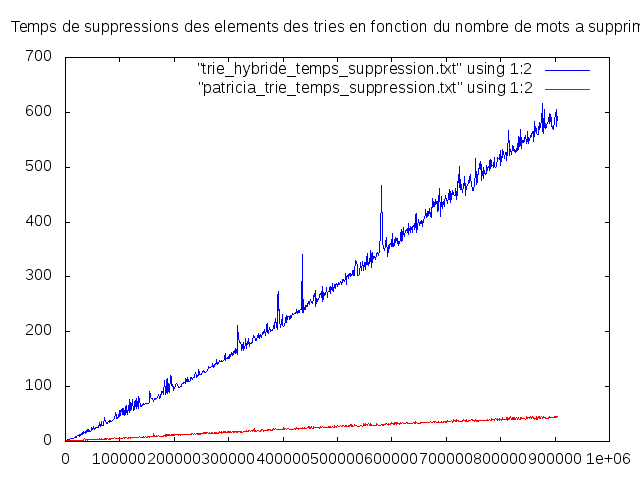
\includegraphics{../comparaison/courbe_temps_suppression.png}
\begin{figure}[!htbp]
\caption{Courbe du temps de calcul en fonction du nombre de suppression}
\end{figure}

\section{Profondeur moyenne des structures}
Cette étude de la profondeur des structures permet de mettre en évidence l'évolution de la profondeur moyenne des structures
suivant le nombre de mots contenus. Nous avons chargé les œuvres de Shakespeare avec un pas de 1000 et en calculant la profondeur
moyenne entre ces ajouts.\\
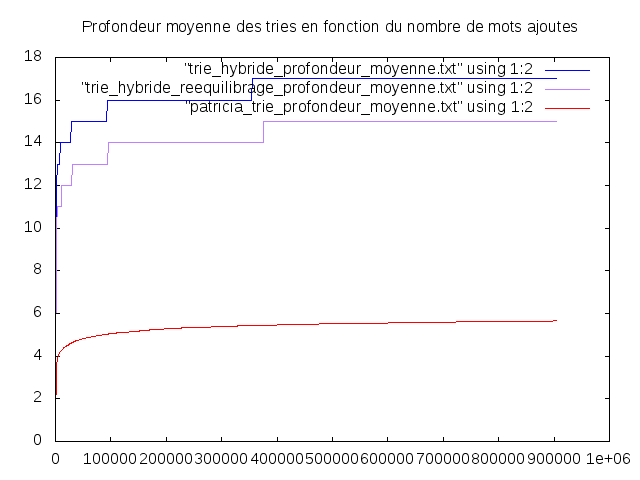
\includegraphics{../comparaison/courbe_profondeur_moyenne.png}
\begin{figure}[!htbp]
\caption{Courbe de la profondeur moyenne en fonction du nombre d'ajouts}
\end{figure}
\section{Hauteur}
De la même manière que pour le calcul de la profondeur moyenne, nous avons chargé les œuvres et Shakespeare avec un pas de 1000
et en calculant la hauteur entre ces ajouts.\\
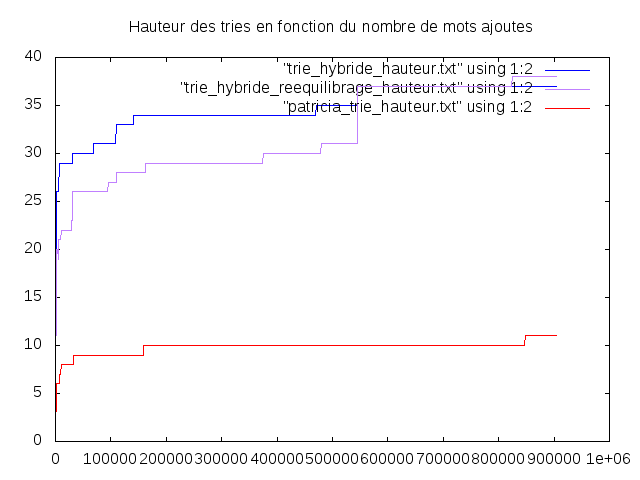
\includegraphics{../comparaison/courbe_hauteur.png}
\begin{figure}[!htbp]
\caption{Courbe de la hauteur en fonction du nombre d'ajouts}
\end{figure}

\end{document}
